%%%%%%%%%%%%%%%%%%%%%%%%%%%%%%%%

\documentclass[11pt,a4paper]{article}
\usepackage{times}
\usepackage[utf8]{inputenc}
\usepackage[croatian]{babel}
\usepackage[T1]{fontenc} % Latin Modern

%%%%%%%%%%%%%%%%%%%%%%%%%%%%%%%%


%%%%%%%%%%%%%%%%%%%%%%%%%%%%%%%%
%%%%%%%%  MATEMATICKI PAKETI %%%%%%%%%%%
%%%%%%%%%%%%%%%%%%%%%%%%%%%%%%%%

\usepackage{amsmath}
\usepackage{amsfonts}
\usepackage{amssymb}
\usepackage{esvect}


%%%%%%%%%%%%%%%%%%%%%%%%%%%%%%%%

%%%%%%%%%%%%%%%%%%%%%%%%%%%%%%%%
%%%%%%%%%% PAKETI ZA SLIKE  %%%%%%%%%%%%
%%%%%%%%%%%%%%%%%%%%%%%%%%%%%%%%

\usepackage{graphicx}
\usepackage{float}
\usepackage[hidelinks]{hyperref}
\usepackage{caption}
\usepackage{subcaption}
\usepackage{booktabs}
\usepackage{mwe}

%%%%%%%%%%%%%%%%%%%%%%%%%%%%%%%%

%%%%%%%%%%%%%%%%%%%%%%%%%%%%%%%%
%%%%%%%%%    PRORED 1.5   %%%%%%%%%%%%%%
%%%%%%%%%%%%%%%%%%%%%%%%%%%%%%%%

\renewcommand{\baselinestretch}{1.5}

%%%%%%%%%%%%%%%%%%%%%%%%%%%%%%%%


%%%%%%%%%%%%%%%%%%%%%%%%%%%%%%%%
%%%%%%%%%% TABLICA - ANTUN %%%%%%%%%%%%
%%%%%%%%%%%%%%%%%%%%%%%%%%%%%%%%

\usepackage{array}
\usepackage{multirow}
\newcolumntype{C}[1]{>{\centering\let\newline\\\arraybackslash\hspace{0pt}}m{#1}}
\newcolumntype{L}[1]{>{\raggedright\let\newline\\\arraybackslash\hspace{0pt}}m{#1}}
\newcolumntype{R}[1]{>{\raggedleft\let\newline\\\arraybackslash\hspace{0pt}}m{#1}}
\usepackage{ctable}

%%%%%%%%%%%%%%%%%%%%%%%%%%%%%%%%

%%%%%%%%%%%%%%%%%%%%%%%%%%%%%%%%
%%%%%%%%%% TABLICA - MARTINA %%%%%%%%%%%
%%%%%%%%%%%%%%%%%%%%%%%%%%%%%%%%

\makeatletter
\renewcommand*\env@matrix[1][\arraystretch]{%
  \edef\arraystretch{#1}%
  \hskip -\arraycolsep
  \let\@ifnextchar\new@ifnextchar
  \array{*\c@MaxMatrixCols c}}
\makeatother



%%%% LATEX KOD ZA KORISTENJE TABLICE %%%%
%%% PRIMJER %%%

%\setlength\extrarowheight{1pt}
%\begin{table}[h]
%\centering
%\caption{Tablica s prikazom }
%\label{prva}
%\begin{tabular}{|l|c|}
%\hline
%\textbf{txt} &  \\ \hline 
%txt & txt    \\ 
%txt & txt   \\ \hline
%txt & txt    \\ \hline
%\end{tabular}
%\end{table}

%%%%%%%%%%%%%%%%%%%%%%%%%%%%%%%%


%%%%%%%%%%%%%%%%%%%%%%%%%%%%%%%%
%%%%%%% DIO ZA UNOS ISJECAKA KODA %%%%%%%%
%%%%%%%%%%%%%%%%%%%%%%%%%%%%%%%%

\usepackage{listings}
\usepackage{color}
 
\definecolor{codegreen}{rgb}{0,0.6,0}
\definecolor{codegray}{rgb}{0.5,0.5,0.5}
\definecolor{codepurple}{rgb}{0.58,0,0.82}
 
\lstdefinestyle{mystyle}{   
    commentstyle=\color{codegreen},
    keywordstyle=\color{blue},
    numberstyle=\tiny\color{codegray},
    stringstyle=\color{codepurple},
    basicstyle=\footnotesize,
    breakatwhitespace=false,         
    breaklines=true,                 
    captionpos=b,                    
    keepspaces=true,                 
    numbers=left,                    
    numbersep=5pt,                  
    showspaces=false,                
    showstringspaces=false,
    showtabs=false,                  
    tabsize=1
}
 
\lstset{style=mystyle}

%\lstinputlisting[language=Matlab, firstline=1, lastline=4, numbers=left, frame=single, label={lst:prvi}, caption={Diskretizacija sustava korištenjem Matlaba}, captionpos=b]{peti.m} 

%%%%%%%%%%%%%%%%%%%%%%%%%%%%%%%%


%----------------------------
% za uredjenje stranice
\usepackage[left=2.5cm,right=2.5cm,top=2.5cm,bottom=2.5cm]{geometry}
\usepackage{fancyhdr}
\pagestyle{fancy} 
\lhead{\leftmark}
\rhead{\rightmark}
\usepackage{titlesec} %za točku iza broja sectiona
\titleformat{\section}{\huge\bfseries}{\thetitle.\quad}{0em}{}
\titleformat{\subsection}{\LARGE\bfseries}{\thetitle.\quad}{0em}{}
\titleformat{\subsubsection}{\Large\bfseries}{\thetitle.\quad}{0em}{}
\titleformat{\paragraph}
{\normalfont\large\bfseries}{\thetitle.\quad}{1em}{}
\titlespacing*{\paragraph}
{0pt}{3.25ex plus 1ex minus .2ex}{1.5ex plus .2ex}
\setcounter{secnumdepth}{5}

\usepackage{indentfirst} %uvlacenje prvog paragrafa
% primjer pozivanja sectiona
% \section*{UVOD} \pdfbookmark{UVOD}{section:UVOD}

\usepackage{tocloft}
\usepackage{import}
\usepackage{standalone}
\graphicspath{{Identifikacija/figures/}} 

\hypersetup{
  colorlinks   = true, %Colours links instead of ugly boxes
  urlcolor     = black, %Colour for external hyperlinks
  linkcolor    = black, %Colour of internal links
  citecolor   = blue %Colour of citations
}

\usepackage{subcaption}
\usepackage{lscape}
\begin{document}

Određivanje parametara neizostavan je dio postupka modeliranja svakog sustava. Većinu parametara, kao što su masa i duljina, određuje se izravnim metodama, kao što su vaganje i mjerenje. Ostale parametre potrebno je odrediti eksperimentalnim putem. U prethodnom poglavlju izvedena je prijenosna funkcija modela (\ref{eq:tf}) u ovisnosti o parametrima $\zeta_{mm}$, $\omega_{mm}$ i $I_{yy}$, odnosno u ovisnosti o prigušenju sustava, nazivnoj frekvenciji i momentu tromosti (pomične mase). Ti su parametri nepoznati te ih je potrebno identificirati. 

\medskip

Identifikacija sustava je postupak određivanja matematičkog modela sustava, kao i njegovih parametara, na temelju mjerenja ulazno/izlaznih signala sustava. Odnosno to je eksperimentalna analiza sustava \cite{te}.

\subsection{Identifikacija dinamike pokretnih masa}

Identifikaciju parametara započinjemo odabirom modela. Pretpostavlja se kako dinamika koračnog sustava masa prati $PT_{2}S$ ponašanje (\ref{eq:pt2s}). $PT_{2}S$ član je sustav drugog reda s konjugirano-kompleksnim parom polova i bez nula \cite{aupr}. Za potrebe identifikacije izrađena je \textit{Matlab Simulink shema} koja ostvaruje ponašanje algoritma upravljanja pozicijom motora pokretanog na \textit{STM} kontroleru. U shemi su postavljeni generatori pulsa koji simuliraju takt vremenskog brojača (\textit{timer-a}) na \textit{STM} kontroleru. Na temelju toga se u određenim vremenskim trenutcima generira impuls koji simulira korak okreta motora. U slučaju da se motor mora gibati većom brzinom, pulsevi se generiraju češće. 400 pulseva jednako je \textit{8 cm} hoda motora. Odziv sustava, odnosno dinamike mase koju je potrebno identificirati, prikazan je Slikom \ref{fig:masa} u nastavku:

\begin{figure}[H]
	\centering
	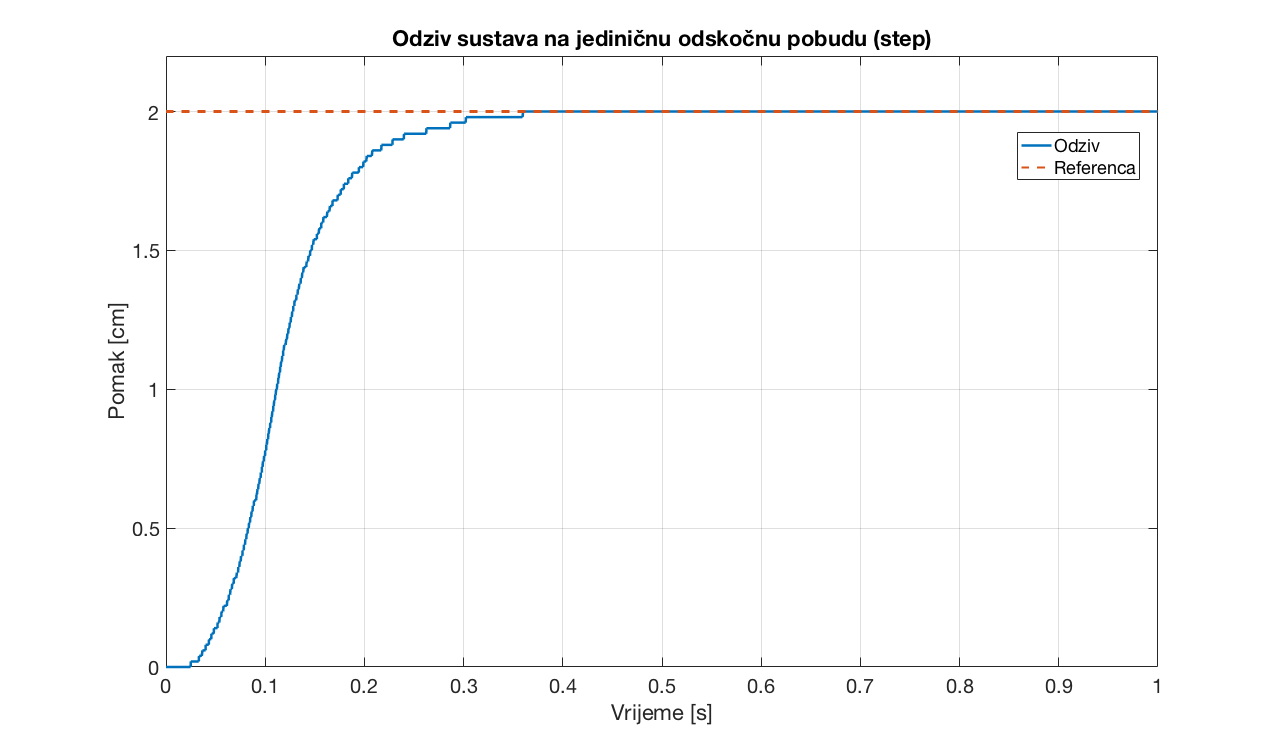
\includegraphics[scale=0.25]{dinamika_masa}
	\caption{Dinamika pomične mase}
	\label{fig:masa}
\end{figure}


Identifikacija započinje proračunom relativnog koeficijenta prigušenja $\zeta_{mm}$. $\zeta_{mm}$ je glavni čimbenik u $PT_{2}S$ članu koji određuje oscilatornost sustava, dok prirodna frekvencija neprigušenih oscilacija $\omega_{n}$ određuje brzinu odziva sustava \cite{aupr}. Pozivom \textit{Matlab} naredbe \textit{stepinfo} na izlazni signal sustava, dobije se informacija o vremenima porasta (\ref{eq:tr}), prvog maksimuma (\ref{eq:tm}) te smirivanja (\ref{eq:te}) koji su potrebni za daljnji proračun parametara. 

\medskip

Vrijeme porasta $t_{r}$ definira se kao vrijeme za koje prijelazna funkcija \textit{y} poraste od vrijednosti $0.1y(\infty)$ na vrijednost $0.9y(\infty)$, gdje $y(\infty)$ označava vrijednost koju funkcija \textit{y} poprima u stacionarnom stanju (njezina konačna vrijednost) te se računa prema izrazu (\ref{eq:tr}):
\begin{equation}
t_{r} \approx \frac{1.8}{\omega_{mm}}
\label{eq:tr}
\end{equation}


Vrijeme prvog maksimuma $t_{m}$ je vrijeme pri kojem se pojavljuje prvo maksimalno nadvišenje:
\begin{equation}
t_{m} = \frac{\pi}{\omega_{mm}\sqrt{1 - \zeta_{mm}^{2}}}
\label{eq:tm}
\end{equation}

Vrijeme smirivanja (ustaljivanja) $t_{1\%}$ određuje trajanje prijelaznog procesa nakon kojega $y$ odstupa od zadanog iznosa za $1\%$:
\begin{equation}
t_{1\%} \approx \frac{4.6}{\zeta_{mm} \cdot \omega_{mm}}
\label{eq:te}
\end{equation}

Na temelju prethodnih jednadžbi intuitivno je jasno kako se pomnim odabirom fizikalno prihvatljivih parametara $\omega_{mm}$ i $\zeta_{mm}$ može dobiti željeno vladanje sustava. Kombinacijom jednadžbi (\ref{eq:tr}) i (\ref{eq:te}) slijedi izraz za proračun prigušenja $\zeta_{mm}$:
\begin{equation}
\zeta_{mm} = 2.556 \frac{t_{r}}{t_{1\%}}
\label{eq:zeta}
\end{equation}

$\omega_{mm}$ se računa koristeći preostalu jednadžbu (\ref{eq:tm}). Uz $t_{r} = 0.139 \ [s]$, $t_{m} = 0.638 \ [s]$ i $t_{1\%} = 0.383 \ [s]$ slijedi da su $\zeta_{mm} = 0.925$, a $\omega_{mm} = 12.992 \ [s^{-1}]$. Simulirajući odziv (\ref{eq:pt2s}) člana s ovim parametrima uočena je potreba za ubrzanjem dobivenog odziva. To je dovelo do dodatnog eksperimentalnog ugađanja parametra $\omega_{mm}$ koji direktno utječe na brzinu odziva, te je on u konačnici jedak $\omega_{mm} = 17.992 \ [s^{-1}]$. Identificirana dinamika pomičnih masa prikazana je Slikom (\ref{fig:masa_din}), dok je konačna prijenosna funkcija jednaka (\ref{eq:mase_tf}):

\begin{equation}
\boxed{
\frac{x_{i}}{x_{i, ref}}(s) = \frac{1}{3.098\cdot10^{-3}s^{2} + 0.103 s + 1}
}
\label{eq:mase_tf}
\end{equation}

\begin{figure}[H]
	\centering
	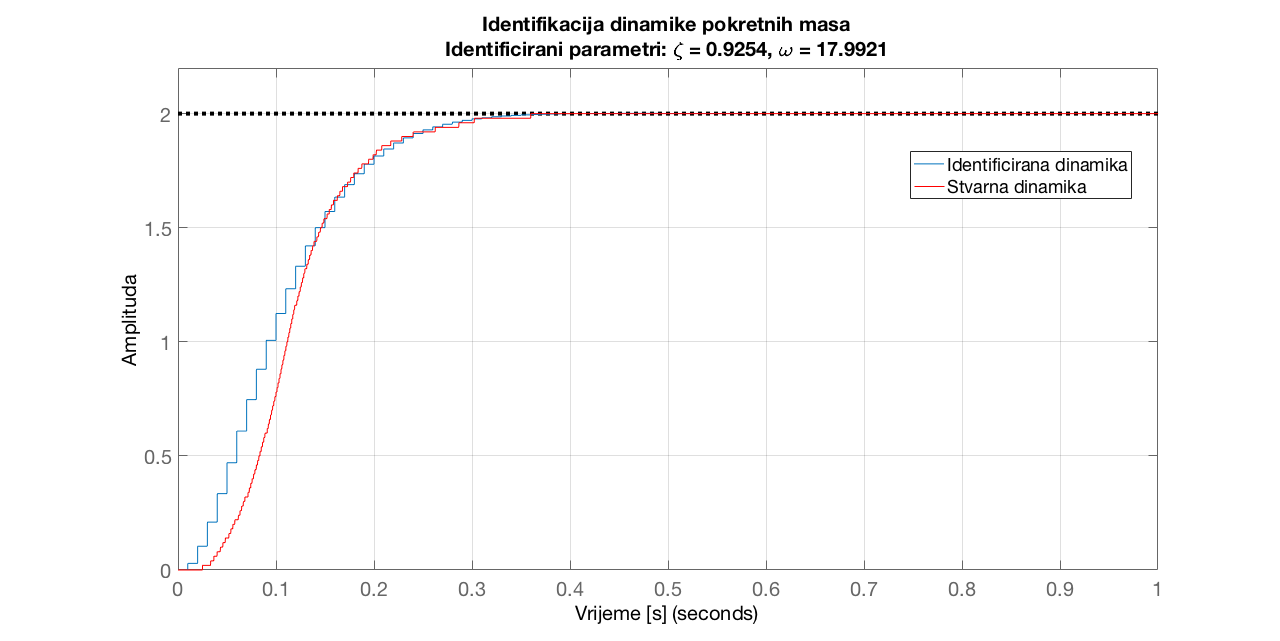
\includegraphics[width=\textwidth]{mase_dinam}
	\caption{Identificirana dinamika pokretnih masa}
	\label{fig:masa_din}
\end{figure}

\subsection{Identifikacija momenta tromosti}

Moment tromosti je mjera tromosti tijela pri rotaciji. On utječe na rotaciju kao što masa utječe na translaciju materijalne točke, stoga ga je izrazito bitno točno identificirati \cite{fiz1}. Određuje se eksperimentalnim putem. 

\medskip

Postupak započinje postavljanjem letjelice na stalak s jednom osi rotacije (\textit{single axis gimbal}). Prvo se provodi eksperiment za \textit{kut poniranja}, a potom za \textit{kut valjanja}. Letjelica se postavlja u horizontalni položaj, tako da je iznos kuta jednak nula, dok se mase postavljaju u proizvoljni krajnji položaj (lijevo ili desno). Potom se letjelica pušta iz početnog položaja te se odzivi snimaju za daljnju identifikaciju. 

\begin{figure}[H]
	\centering
	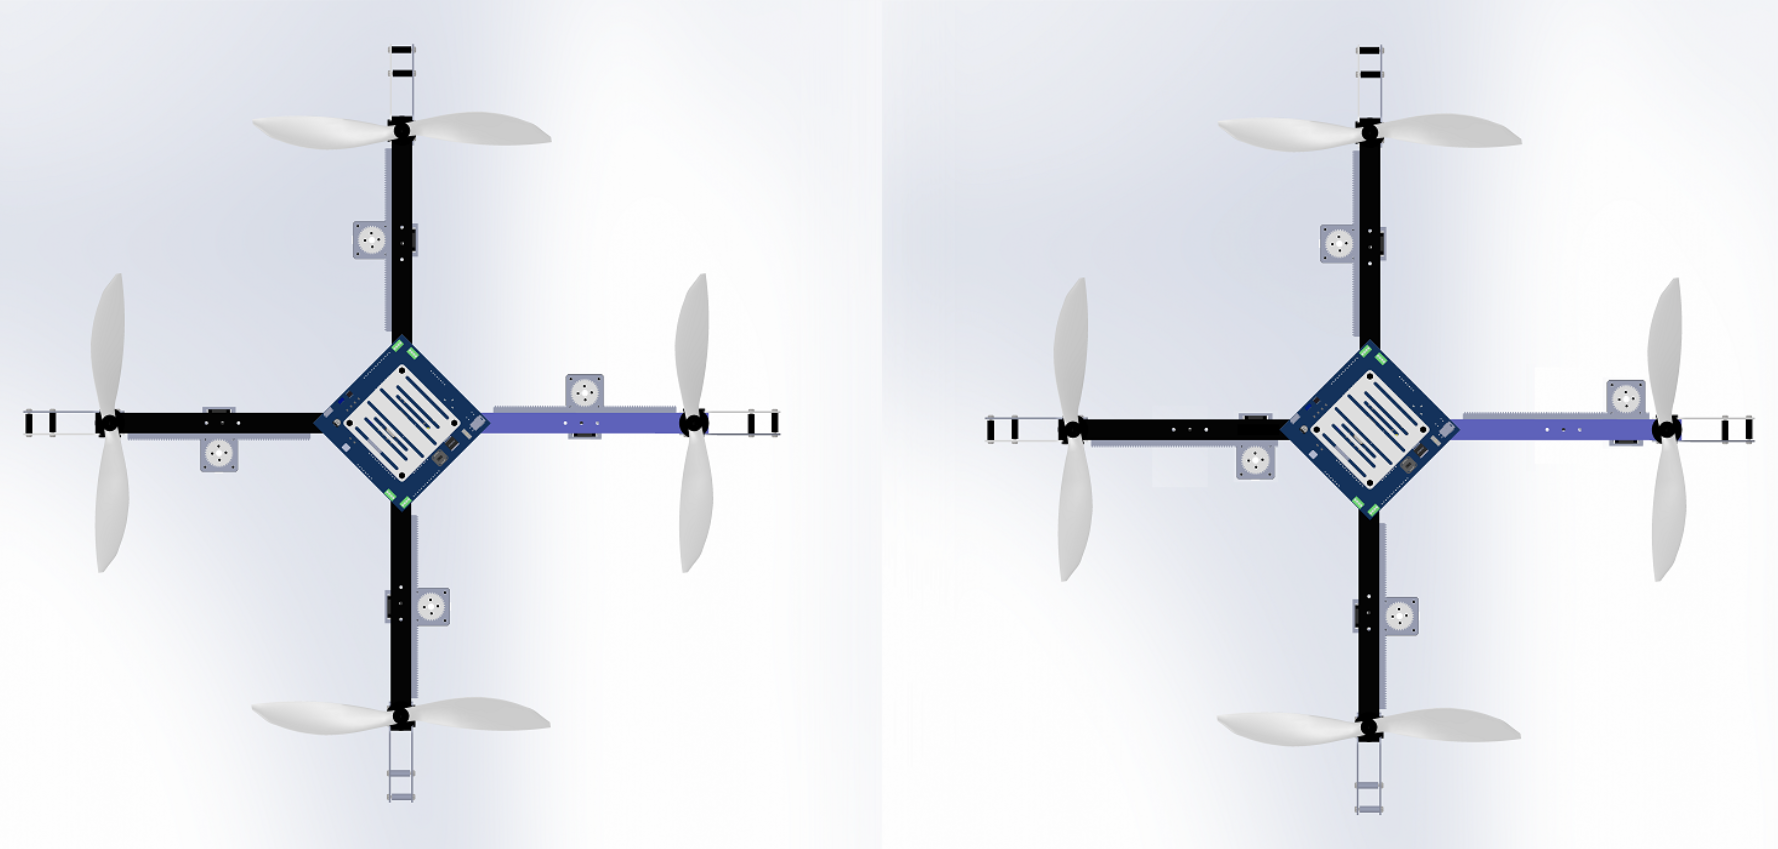
\includegraphics[scale=0.2]{pomak}
	\caption{Prikaz pomaka pomičnih masa za $\Delta x = 8 \ cm$ u svrhu identifikacije momenta tromosti}
	\label{fig:}
\end{figure}


\medskip

U tako kontroliranom okruženju, na letjelicu ne djeluju vanjski poremećaji već samo sila gravitacije. Stoga u izrazu (\ref{eq:Iyyw}) ostaje samo prvi član, dok su ostali jednaki nula:
\begin{equation}
I_{yy} \dot{\omega}_{y} = \sum_{j=1}^{4} M_{fj}  =  \sum_{j=1}^{4} r_{c,j} \times F_{r,j}
\label{eq:Iyyw2}
\end{equation}

gdje su:
\begin{equation}
F_{r,1} = F_{r,2} = F_{r,3} = F_{r,4} = \frac{F_{g}}{4} = \frac{Mg}{4}
\label{eq:F1234}
\end{equation}

\begin{equation}
r_{c1,x} = \ell + \Delta \ell \  \  , \ r_{c2,x} = \Delta \ell \  \ , \  r_{c3,x} = \ell - \Delta x \  \ , \  r_{c4,x} =  \Delta x
\label{eq:rcj}
\end{equation}

gdje je $\Delta \ell = \mu(x_{1}  + x_{3})$.

Uvrštavanjem (\ref{eq:Fg}),(\ref{eq:F1234}) i (\ref{eq:rcj}) u (\ref{eq:Iyyw2}) slijedi:
\begin{equation}
 I_{yy}\dot{\omega}_{y} = mg(x_{1} + x_{3})
 \label{eq:Iyyw3}
 \end{equation} 
 
 Ali s obzirom da se mase pomiču za jednaku vrijednost, vrijedi jednakost:
 \begin{equation}
 x_{1} = x_{3} = 2\cdot\Delta x
 \label{eq:x1xx3}
 \end{equation}
pa slijedi:
\begin{equation}
I_{yy} \dot{\omega}_{y} = 2mg\Delta x = u
\label{eq:upr}
\end{equation}

Prelaskom u Laplaceovu domenu, te izražavanjem parametra $\omega_{y}$ koji je poznat iz snimljenih odziva, slijedi sustav koji je potrebno modelirati, odnosno koji se koristi pri identifikaciji:
\begin{equation}
\omega_{y} = \frac{2mg \Delta x}{I_{yy}} \frac{1}{s} = \frac{u}{I_{yy}} \frac{1}{s} = u \cdot K_{identif.} \cdot \frac{1}{s}
\label{eq:wy}
\end{equation}
\medskip
gdje je $K_{identif.}$ nepoznati parametar koji se identificira te je jednak $\frac{1}{I_{yy}}$, dok je $u$ poznati upravljački signal koji se koristi kao pobuda sustava identifikacije.

Identifikacija se provodi u programskom okruženju \textit{Matlab} koristeći \textit{fminsearch} metodu. Eksperimentalna analiza ponovljena je na četiri skupa mjerenja, identificirani odzivi i parametri prikazani su Slikom (\ref{fig:Iyy}):   
    



\begin{figure}[H]
	\centering
	\begin{subfigure}{.5\textwidth}
		\centering
		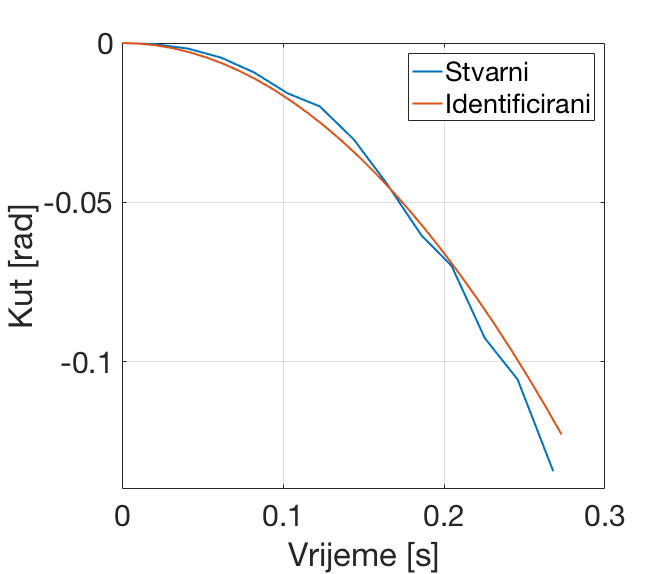
\includegraphics[width=1\linewidth]{1}
		\caption{$I_{yy} = 0.0990 \ kg \cdot m^{2}$}
		\label{fig:mj1}
	\end{subfigure}%
	\begin{subfigure}{.5\textwidth}
		\centering
		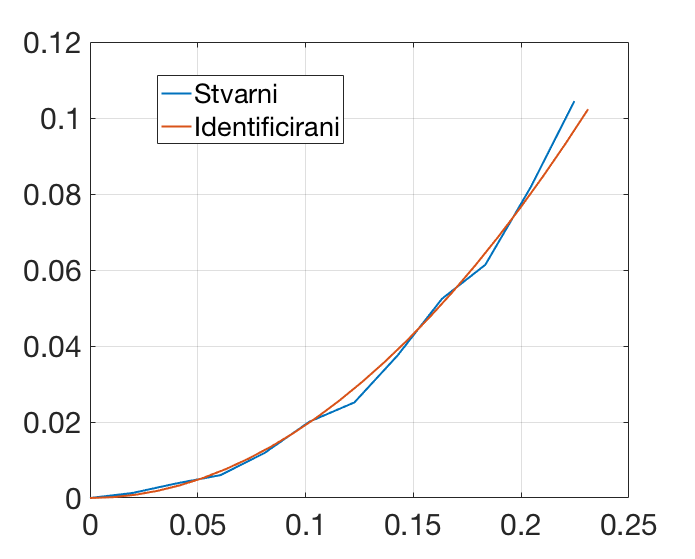
\includegraphics[width=1\linewidth]{2}
		\caption{K$I_{yy} = 0.08515 \ kg \cdot m^{2}$}
		\label{fig:mj2}
	\end{subfigure}
	\begin{subfigure}{.5\textwidth}
		\centering
		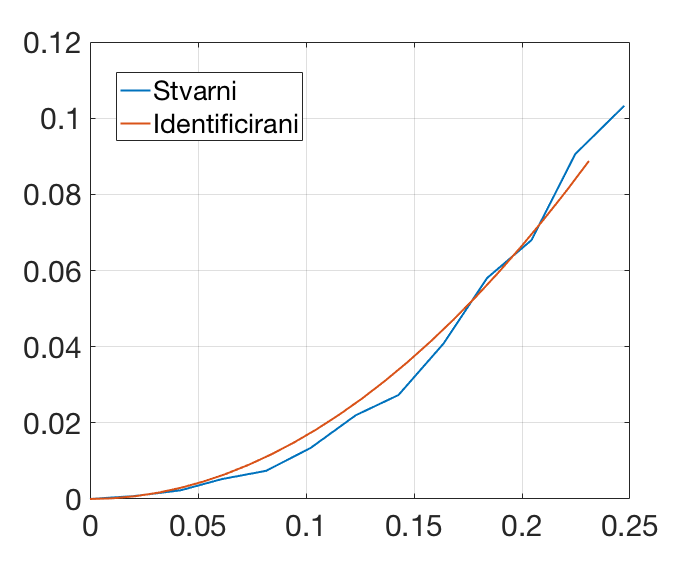
\includegraphics[width=1\linewidth]{3}
		\caption{$I_{yy} = 0.0981 \ kg \cdot m^{2}$}
		\label{fig:mj3}
	\end{subfigure}%
	\begin{subfigure}{.5\textwidth}
		\centering
		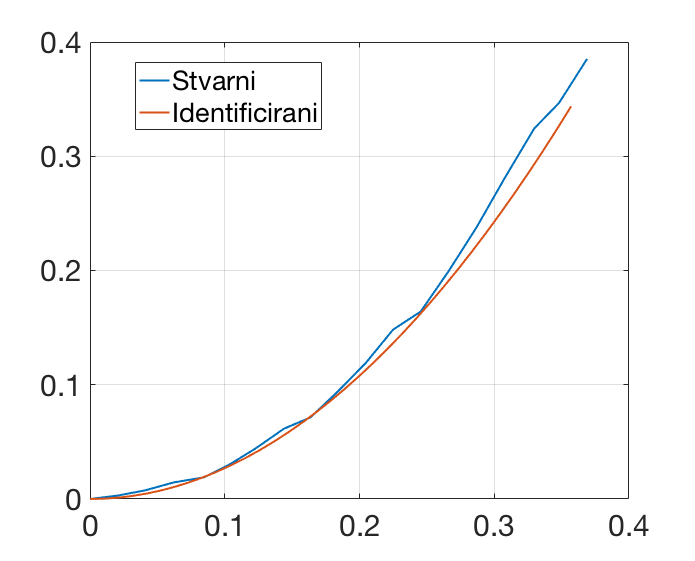
\includegraphics[width=1\linewidth]{4}
		\caption{$I_{yy} = 0.06055 \ kg \cdot m^{2}$}
		\label{fig:mj4}
	\end{subfigure}
	
	\caption{Rezultat identifikacije momenta tromosti}
	\label{fig:Iyy}
\end{figure} 



Konačan iznos momenta tromosti $I_{yy}$ odabiremo kao srednju vrijednost dobivenih rezultata:

\begin{equation}
\boxed{
I_{yy} = 0.0857 \ kg \cdot m^{2}
}
\label{eq:Iyy}
\end{equation}


\newpage

\subsection{Parametri modela letjelice}




\setlength\extrarowheight{1pt}
\begin{table}[h]
\centering
\caption{Parametri modela letjelice}
\label{params}
\begin{tabular}{lll}
\hline
\textbf{Oznaka} &  \textbf{Iznos}  &  \textbf{Opis}   \\ \hline 
$I_{xx}$ & $0.0857 \ kgm^{2}$ & Moment tromosti cijelog sustava letjelice (\textit{kut valjanja})   \\ 
$I_{yy}$ & $0.0857 \ kg m^{2}$ &  Moment tromosti cijelog sustava letjelice (\textit{kut poniranja})\\ 
$m$ & $0.208 \ kg$ &  Masa pokretne mase    \\ 
$M$ & $2.083 \ kg$ & Ukupna masa letjelice      \\ 
$b_{f}$ & $8.54858e-6 \ kgm$& Konstanta potiska motora     \\ 
$b_{m}$ & $0.01$& Momentna konstanta motora     \\ 
$ L$ & $0.2520 \ m $ &  Duljina kraka letjelice    \\ 
$\omega_{mm} $ & $ 17.9921 \ rad\/s$ & Nazivna frekvencija kliznog mehanizma pokretnih masa     \\
$\zeta_{mm} $ & $ 0.9254 \ rad\/s$ & Faktor prigušivanja kliznog mehanizma pokretnih masa      \\  
$T_{r} $ & $ 0.2 \ s$ &  Vremenska konstanta rotora    \\
$\Delta \ell $ & $\pm0.08 \ m $ &  Maksimalan hod pokretnih masa    \\  
$z_{m} $ & $ 0$ & Vertikalan pomak masa s obzirom na ishodište     \\ 
$T_{s} $ & $ 0.01 \ s$ &  Vrijeme uzorkovanja diskretnog sustava    \\ \hline
\end{tabular}
\end{table}



\end{document}